\begin{frame}
  \begin{center}
    {\color{Maroon}\Huge Introduction}
  \end{center}
\end{frame}

%% put section outline here
\begin{frame}{Introduction}{Outline}
  \begin{enumerate}
  \item The shift in speech based user interfaces
  \item Building applications on the information rich speech signal
  \item The Speech Recognition Case Study
    \begin{itemize}
    \item From rule-based systems to data-driven system
    \item Impact of speech recognition technologies across languages and domains
    \item What is under the hood for speech recognition technologies?
    \item Building various ASR module and the impact of data
    \end{itemize}
  \item Building ASR Systems in New Languages
    \begin{itemize}
    \item Building from ASR systems from scratch
    \item Is there room for sharing data from other languages?
    \end{itemize}
  \item Building ASR Systems in New Domain
    \begin{itemize}
    \item Adaptation of an existing ASR system
    \end{itemize}
  \end{enumerate}
\end{frame}

\begin{frame}{Speech based user interfaces}{}
\begin{columns}[T]
    \column{2.5in}
     \alert{Star Trek's Universal Translator} [Wikipedia] -  \dots used in the late 22nd century on 
     Earth for the \alert{instant translation of well-known Earth languages}. Gradually, with 
     the removal of language barriers, Earth's disparate cultures came to terms of 
     universal peace. Translations of \alert{previously unknown languages}, such as those of 
     aliens, required more difficulties to be overcome. 
     \column{2in}
     \vspace{1cm}
     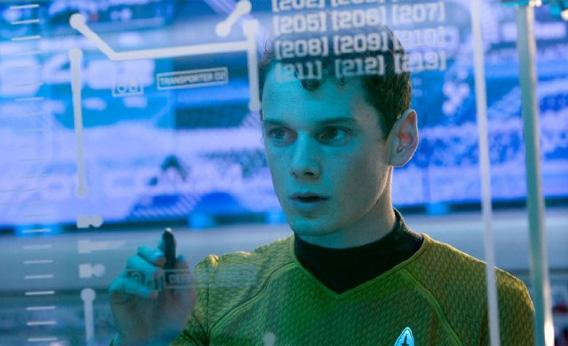
\includegraphics[height=30mm]{figures/startrek_comp}
  \end{columns}
\end{frame}

\begin{frame}{Speech based user interfaces}{}
\begin{columns}[T]
    \column{3in}
     \alert{Star Trek: The Next Generation Technical Manual} [Wikipedia] -  \dots the Universal Translator 
     is an "extremely sophisticated computer program" which functions by \alert{analyzing the patterns} of an unknown 
     foreign language, starting from \alert{a speech sample of two or more speakers in conversation}. The more extensive 
     the conversational sample, the more accurate and reliable is the "translation matrix," enabling instantaneous 
     conversion of verbal utterances or written text between the alien language and Federation Standard.
     \column{1in}
     \vspace{1.2cm}
     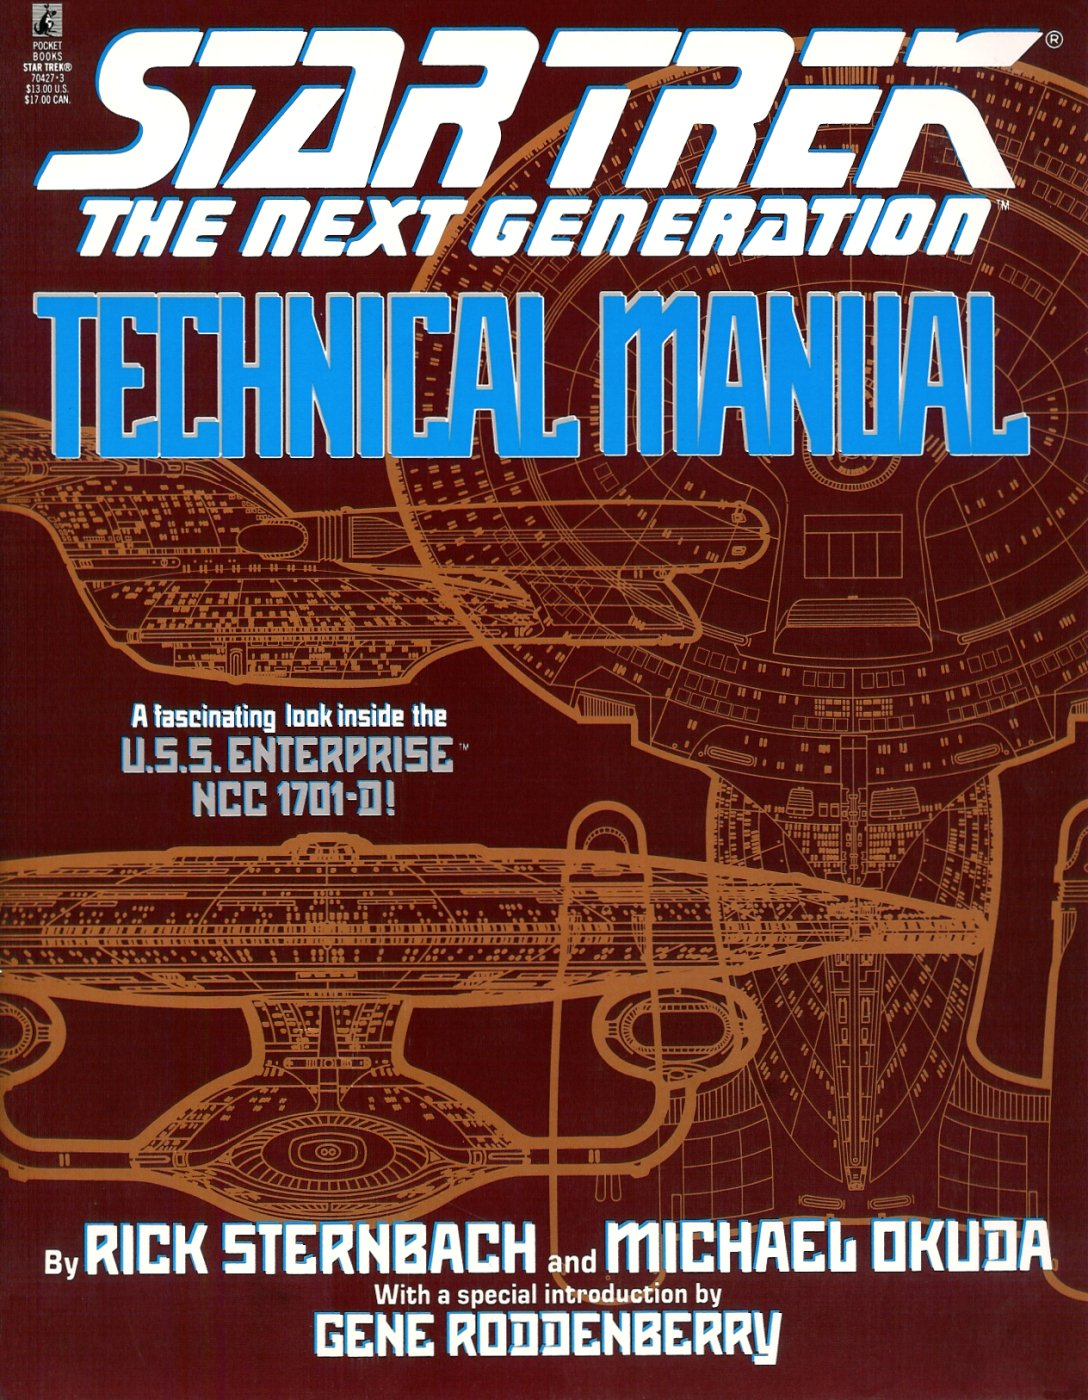
\includegraphics[height=40mm]{figures/startrek_manual}
  \end{columns}
\end{frame}

% Various applications that can be built on the speech signal
\begin{frame}{Building applications on the speech signal}
   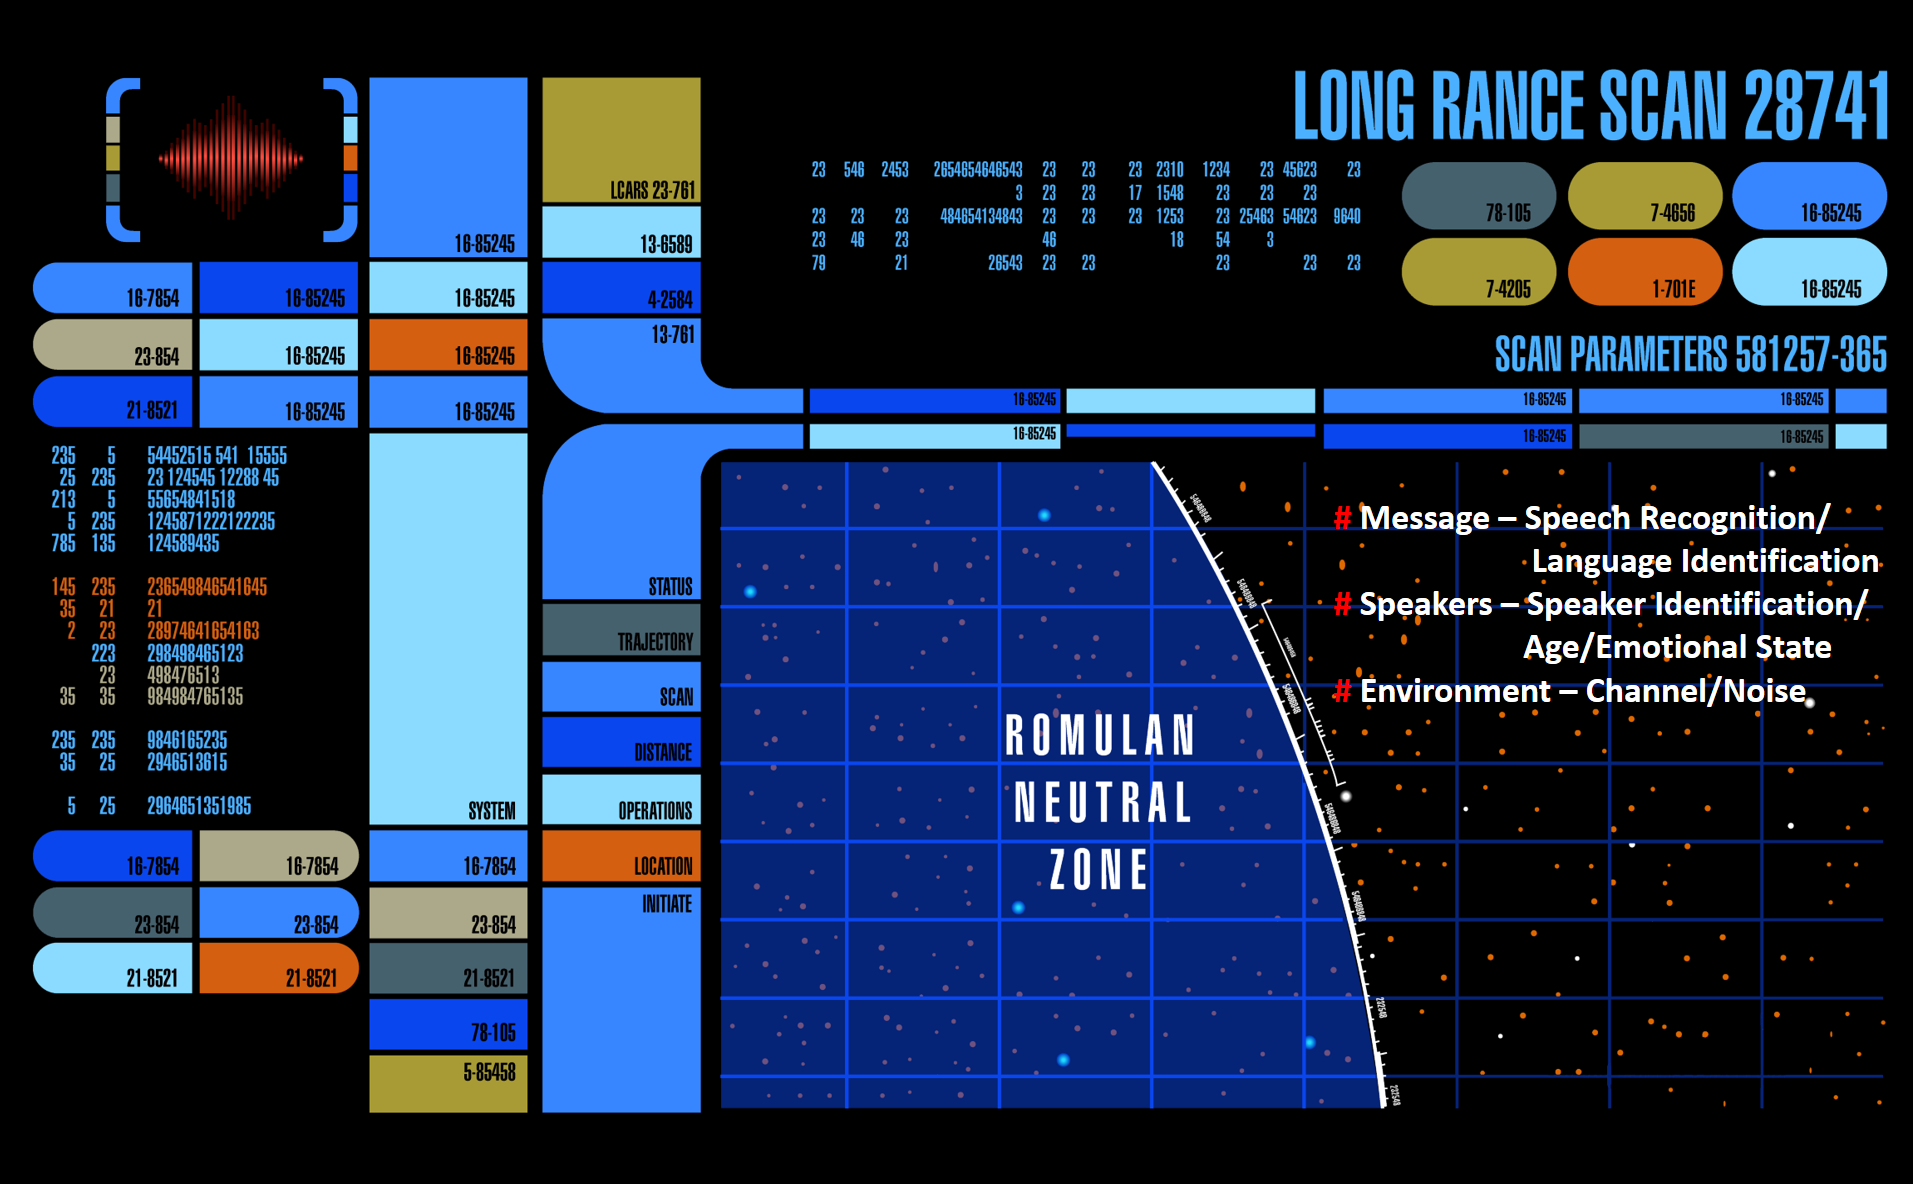
\includegraphics[height=70mm]{figures/technologies}
\end{frame}

% Show the progress from rule based to data based technologies
\begin{frame}{The Speech Recognition Case Study}
\end{frame}

% Show the progress in building technolgies acorss languages
\begin{frame}{Impact of speech recognition technologies across languages and domains}
\end{frame}

% What does it take 
\begin{frame}{What is under the hood for speech recognition technologies?}
\end{frame}
